\subsection{Completed transfer curves and extraction limitations}
All five Sentaurus Process simulations at activation temperatures
$800$, $850$, $900$, $950$ and $1000\,^\circ$C completed
successfully. Each final device structure was subsequently simulated
in Sentaurus Device at $V_{DS}=0.1$ and $1.2$ V, giving ten
completed $I_D$--$V_G$ sweeps. The structures and raw sweep outputs
are retained in the university Sentaurus Workbench project
\texttt{SOI\_nMOSFET\_Part\_3}. The exported 35-point gate sweeps per
drain-bias case were analyzed with Python; repeated initialization
points at $V_{GS}=-0.5$ V were discarded by retaining the final
current for each gate voltage. The results summarized here are
transcribed from the 24 October 2026 analysis output.

\paragraph{Definition of metrics and their domain.}
To remain consistent with the Part 2 analysis, the
constant-current threshold $V_{\mathrm{TH,CC}}$ uses
$|I_D|=10^{-7}$ in \emph{exported current units} and linear
interpolation in $\log_{10}|I_D|$ between adjacent gate-voltage
samples. A threshold is reported only if that criterion is crossed
\emph{within} the simulated $V_{GS}$ interval of $-0.5$ to $1.2$ V.
The apparent SS is extracted by least-squares fitting
$\log_{10}|I_D|$ over $-0.20\le V_{GS}\le0.05$ V at
$V_{DS}=0.1$ V and computing $1000/\mathrm{slope}$ in mV/dec.
A high linear-fit $R^2$ does not necessarily mean that this
fixed window is in true weak inversion, particularly for the
high-leakage devices.
$I_{\mathrm{ON}}=|I_D|(V_{GS}=V_{DS}=1.2\ \mathrm V)$,
and $I_{\mathrm{OFF}}=|I_D|(V_{GS}=0,V_{DS}=1.2\ \mathrm V)$.
The two-dimensional current-width normalization has not yet been
verified, so all current magnitudes below are labelled
\emph{exported current units}, not amperes or amperes per micrometre.

\begin{table}[H]\centering\small
\caption{Part 3 values extracted from completed Sentaurus sweeps.
N/A denotes a current criterion outside the measured gate-voltage range,
not a missing or failed simulation.}
\resizebox{\linewidth}{!}{%
\begin{tabular}{@{}rrrrrrrr@{}}\toprule
Anneal ($^\circ$C) & $V_{\mathrm{TH,CC}}(0.1)$ (V) &
$V_{\mathrm{TH,CC}}(1.2)$ (V) &
SS (mV/dec) & $I_{\mathrm{ON}}$ &
$I_{\mathrm{OFF}}$ & $I_{\mathrm{ON}}/I_{\mathrm{OFF}}$ &
DIBL (mV/V)\\\midrule
800  & $-0.3016$ & N/A & 210.62 & $1.18657\times10^{-3}$ & $7.31697\times10^{-5}$ & 16.22 & N/A\\
850  & $-0.4518$ & N/A & 276.73 & $1.29606\times10^{-3}$ & $1.13044\times10^{-4}$ & 11.47 & N/A\\
900  & N/A & N/A & 299.56 & $1.36570\times10^{-3}$ & $1.28212\times10^{-4}$ & 10.65 & N/A\\
950  & N/A & N/A & 347.23 & $1.44048\times10^{-3}$ & $1.55081\times10^{-4}$ & 9.29 & N/A\\
1000 & N/A & N/A & 1037.98 & $1.92229\times10^{-3}$ & $4.95320\times10^{-4}$ & 3.88 & N/A\\
\bottomrule\end{tabular}}
\end{table}

\paragraph{Threshold and DIBL availability.}
At $V_{DS}=1.2$ V, even the minimum current observed in each of
the five simulated gate sweeps exceeds $10^{-7}$: the minimum
increases from $1.1132\times10^{-5}$ at $800\,^\circ$C to
$3.32728\times10^{-4}$ at $1000\,^\circ$C.
The common current range across both drain biases and all
temperatures is only
$3.32728\times10^{-4}$ to $3.95736\times10^{-4}$,
far above the selected subthreshold reference.
Accordingly none of the high-$V_{DS}$ thresholds can be extracted
using the predeclared reference, and
\[
\mathrm{DIBL}_{\mathrm{CC}}=
1000\,\frac{V_{\mathrm{TH,CC}}(0.1\mathrm{\,V})-
V_{\mathrm{TH,CC}}(1.2\mathrm{\,V})}{1.1\mathrm{\,V}}
\]
is not numerically evaluable at any anneal temperature.
Replacing the current criterion with an on-state value would
give a \emph{different} matched-current voltage shift, not the same
subthreshold-threshold DIBL. No extrapolated values are reported.

\paragraph{Temperature dependence of the threshold criterion.}
\begin{figure}[H]\centering
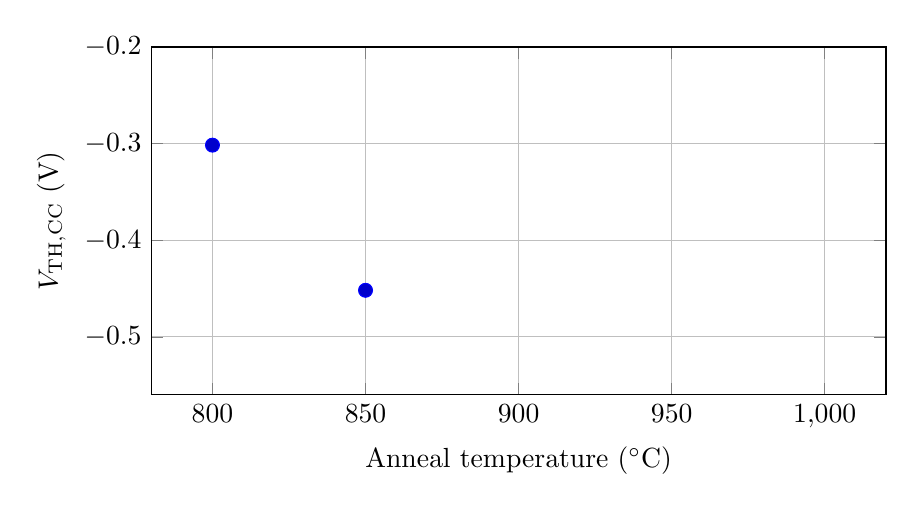
\begin{tikzpicture}
\begin{axis}[width=.90\linewidth,height=6.0cm,
xlabel={Anneal temperature ($^\circ$C)},
ylabel={$V_{\mathrm{TH,CC}}$ (V)},xmin=780,xmax=1020,
xtick={800,850,900,950,1000},ymin=-.56,ymax=-.2,
grid=both]
\addplot+[only marks,mark=*,mark size=2.5pt]
coordinates {(800,-0.3016) (850,-0.4518)};
\end{axis}
\end{tikzpicture}
\caption{Measured low-drain-bias constant-current threshold versus
anneal temperature. Only two of five temperatures cross the chosen
current criterion; the high-$V_{DS}$ thresholds are all unavailable.
No interpolation or trend line is drawn through missing values.}
\end{figure}

\paragraph{Temperature dependence of apparent SS.}
\begin{figure}[H]\centering
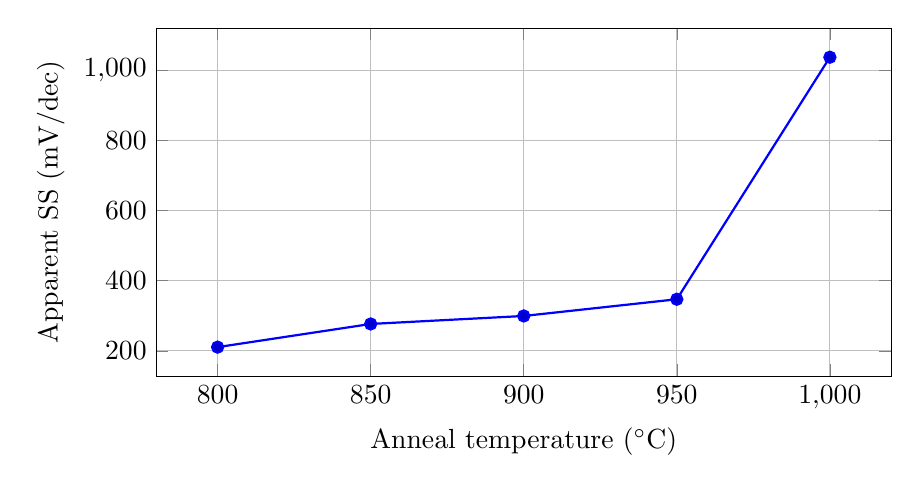
\begin{tikzpicture}
\begin{axis}[width=.90\linewidth,height=6.0cm,
xlabel={Anneal temperature ($^\circ$C)},ylabel={Apparent SS (mV/dec)},
xtick={800,850,900,950,1000},grid=both]
\addplot+[mark=*,thick]
coordinates {(800,210.6228)(850,276.7341)(900,299.5590)(950,347.2256)(1000,1037.9815)};
\end{axis}
\end{tikzpicture}
\caption{Common-window apparent SS at $V_{DS}=0.1$ V.
The high-temperature slope is a fixed-window result, not a demonstrated
weak-inversion subthreshold swing.}
\end{figure}

\paragraph{Temperature dependence of ON current.}
\begin{figure}[H]\centering
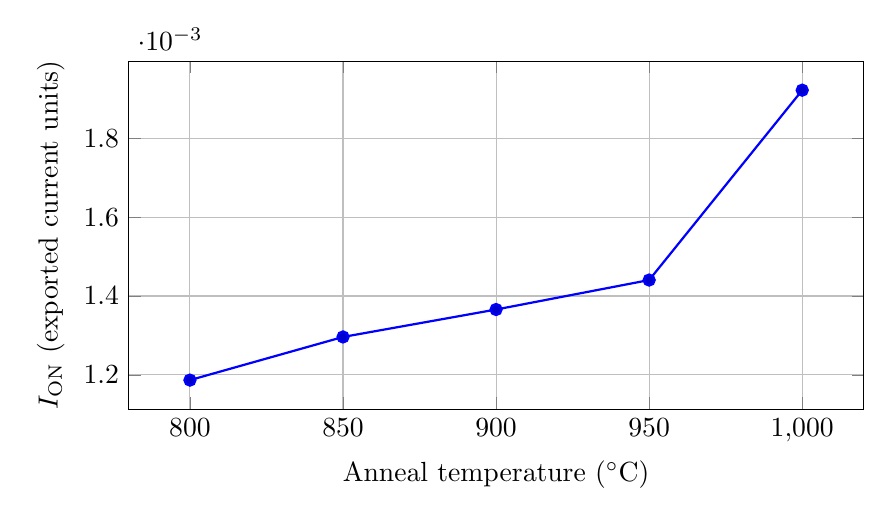
\begin{tikzpicture}
\begin{axis}[width=.90\linewidth,height=6.0cm,
xlabel={Anneal temperature ($^\circ$C)},
ylabel={$I_{\mathrm{ON}}$ (exported current units)},
xtick={800,850,900,950,1000},grid=both]
\addplot+[mark=*,thick]
coordinates {(800,0.00118657)(850,0.00129606)(900,0.00136570)(950,0.00144048)(1000,0.00192229)};
\end{axis}
\end{tikzpicture}
\caption{ON-state drain current at $V_{GS}=V_{DS}=1.2$ V
from the original Sentaurus-exported currents.}
\end{figure}

\paragraph{Temperature dependence of OFF current.}
\begin{figure}[H]\centering
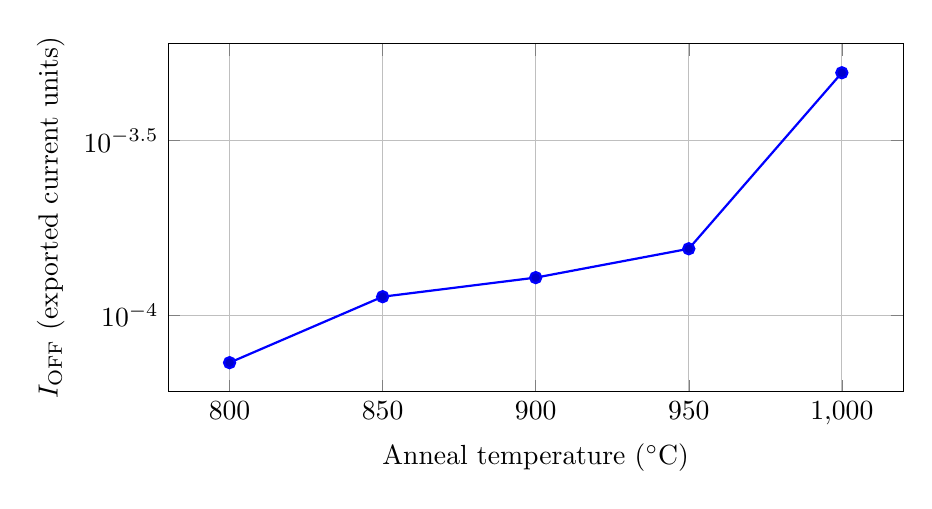
\begin{tikzpicture}
\begin{semilogyaxis}[width=.90\linewidth,height=6.0cm,
xlabel={Anneal temperature ($^\circ$C)},
ylabel={$I_{\mathrm{OFF}}$ (exported current units)},
xtick={800,850,900,950,1000},grid=both]
\addplot+[mark=*,thick]
coordinates {(800,0.0000731697)(850,0.000113044)(900,0.000128212)(950,0.000155081)(1000,0.00049532)};
\end{semilogyaxis}
\end{tikzpicture}
\caption{OFF-state drain current at $V_{GS}=0$ V and
$V_{DS}=1.2$ V, displayed on a logarithmic vertical axis.}
\end{figure}

\paragraph{DIBL criterion: why the numerical plot is unavailable.}
\begin{figure}[H]\centering
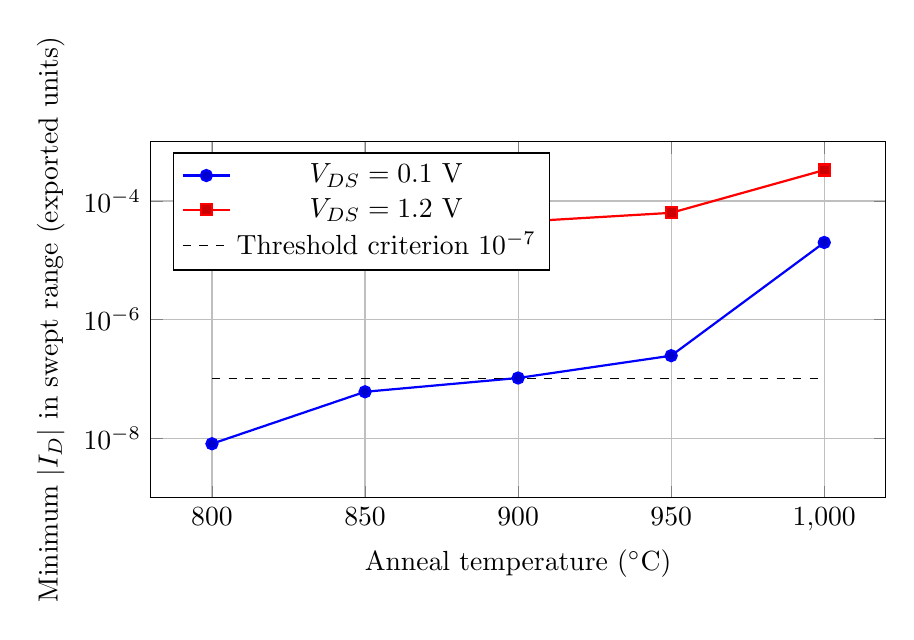
\begin{tikzpicture}
\begin{semilogyaxis}[width=.90\linewidth,height=6.1cm,
xlabel={Anneal temperature ($^\circ$C)},
ylabel={Minimum $|I_D|$ in swept range (exported units)},
xtick={800,850,900,950,1000},
ymin=1e-9,ymax=1e-3,
legend pos=north west,grid=both]
\addplot+[mark=*,thick]
coordinates {(800,8.05874e-9)(850,6.06575e-8)(900,1.03631e-7)(950,2.46313e-7)(1000,1.99863e-5)};
\addlegendentry{$V_{DS}=0.1$ V}
\addplot+[mark=square*,thick]
coordinates {(800,1.1132e-5)(850,3.40328e-5)(900,4.4483e-5)(950,6.32194e-5)(1000,3.32728e-4)};
\addlegendentry{$V_{DS}=1.2$ V}
\addplot+[dashed,black,mark=none]
coordinates {(800,1e-7)(1000,1e-7)};
\addlegendentry{Threshold criterion $10^{-7}$}
\end{semilogyaxis}
\end{tikzpicture}
\caption{Diagnostic replacing an otherwise undefined numerical
DIBL-vs-temperature plot: the minimum current in every high-$V_{DS}$
sweep lies above the $10^{-7}$ reference. Thus this reference-current
DIBL cannot be extracted from the existing bias sweeps.}
\end{figure}

\paragraph{Why larger $I_{\mathrm{ON}}$ alone is insufficient.}
Raising the activation anneal temperature from $800$ to
$1000\,^\circ$C increases the extracted ON current by approximately
$62.0\%$, but increases OFF leakage by a factor of approximately
$6.77$. Meanwhile the apparent SS changes from $210.62$ to
$1037.98$ mV/dec, and the ON/OFF ratio declines from $16.22$
to $3.88$. In these simulations the drive-current improvement is
therefore accompanied by much poorer switching discrimination
and substantially higher off-state conduction. The data are
\emph{consistent with}, but by themselves do not establish,
temperature-induced redistribution of source/drain arsenic,
greater effective junction encroachment, or punch-through.
Direct arsenic-profile comparisons are needed to distinguish
the physical mechanism. Selection of an annealing temperature
requires jointly considering drive, leakage, and electrostatic
control, not maximizing ON current alone.

\paragraph{Required evidence still outstanding.}
Original arsenic-concentration cross-section and/or cutline plots
at $800$ and $1000\,^\circ$C, together with the corresponding
seven-curve $I_D$--$V_D$ output-characteristic comparison,
are not yet included. Current-width normalization likewise
requires verification before physical current units are asserted.
